% Created by tikzDevice version 0.6.2-92-0ad2792 on 2013-05-05 15:31:48
% !TEX encoding = UTF-8 Unicode
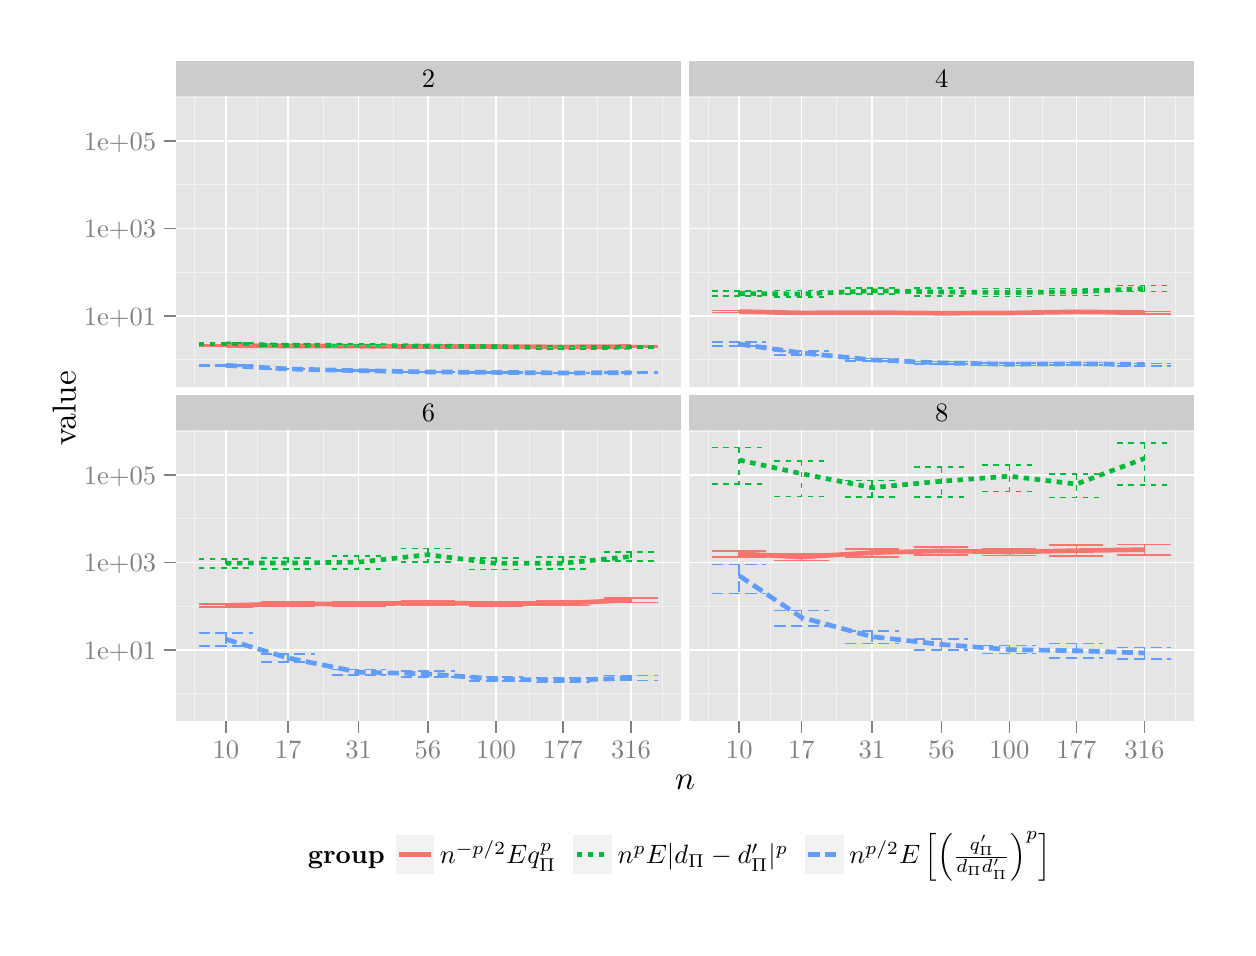
\begin{tikzpicture}[x=1pt,y=1pt]
\definecolor[named]{fillColor}{rgb}{1.00,1.00,1.00}
\path[use as bounding box,fill=fillColor,fill opacity=0.00] (0,0) rectangle (433.62,325.21);
\begin{scope}
\path[clip] (  0.00,  0.00) rectangle (433.62,325.21);
\definecolor[named]{drawColor}{rgb}{1.00,1.00,1.00}
\definecolor[named]{fillColor}{rgb}{1.00,1.00,1.00}

\path[draw=drawColor,line width= 0.6pt,line join=round,line cap=round,fill=fillColor] (  0.00,  0.00) rectangle (433.62,325.21);
\end{scope}
\begin{scope}
\path[clip] ( 53.55,195.47) rectangle (236.06,300.54);
\definecolor[named]{fillColor}{rgb}{0.90,0.90,0.90}

\path[fill=fillColor] ( 53.55,195.47) rectangle (236.06,300.54);
\definecolor[named]{drawColor}{rgb}{0.95,0.95,0.95}

\path[draw=drawColor,line width= 0.3pt,line join=round] ( 53.55,205.20) --
	(236.06,205.20);

\path[draw=drawColor,line width= 0.3pt,line join=round] ( 53.55,236.83) --
	(236.06,236.83);

\path[draw=drawColor,line width= 0.3pt,line join=round] ( 53.55,268.47) --
	(236.06,268.47);

\path[draw=drawColor,line width= 0.3pt,line join=round] ( 53.55,300.11) --
	(236.06,300.11);

\path[draw=drawColor,line width= 0.3pt,line join=round] ( 60.36,195.47) --
	( 60.36,300.54);

\path[draw=drawColor,line width= 0.3pt,line join=round] ( 82.85,195.47) --
	( 82.85,300.54);

\path[draw=drawColor,line width= 0.3pt,line join=round] (106.84,195.47) --
	(106.84,300.54);

\path[draw=drawColor,line width= 0.3pt,line join=round] (132.11,195.47) --
	(132.11,300.54);

\path[draw=drawColor,line width= 0.3pt,line join=round] (156.93,195.47) --
	(156.93,300.54);

\path[draw=drawColor,line width= 0.3pt,line join=round] (181.33,195.47) --
	(181.33,300.54);

\path[draw=drawColor,line width= 0.3pt,line join=round] (205.71,195.47) --
	(205.71,300.54);

\path[draw=drawColor,line width= 0.3pt,line join=round] (229.25,195.47) --
	(229.25,300.54);
\definecolor[named]{drawColor}{rgb}{1.00,1.00,1.00}

\path[draw=drawColor,line width= 0.6pt,line join=round] ( 53.55,221.02) --
	(236.06,221.02);

\path[draw=drawColor,line width= 0.6pt,line join=round] ( 53.55,252.65) --
	(236.06,252.65);

\path[draw=drawColor,line width= 0.6pt,line join=round] ( 53.55,284.29) --
	(236.06,284.29);

\path[draw=drawColor,line width= 0.6pt,line join=round] ( 71.61,195.47) --
	( 71.61,300.54);

\path[draw=drawColor,line width= 0.6pt,line join=round] ( 94.10,195.47) --
	( 94.10,300.54);

\path[draw=drawColor,line width= 0.6pt,line join=round] (119.57,195.47) --
	(119.57,300.54);

\path[draw=drawColor,line width= 0.6pt,line join=round] (144.64,195.47) --
	(144.64,300.54);

\path[draw=drawColor,line width= 0.6pt,line join=round] (169.22,195.47) --
	(169.22,300.54);

\path[draw=drawColor,line width= 0.6pt,line join=round] (193.43,195.47) --
	(193.43,300.54);

\path[draw=drawColor,line width= 0.6pt,line join=round] (218.00,195.47) --
	(218.00,300.54);
\definecolor[named]{drawColor}{rgb}{0.97,0.46,0.43}

\path[draw=drawColor,line width= 1.7pt,line join=round] ( 71.61,210.34) --
	( 94.10,210.19) --
	(119.57,210.13) --
	(144.64,209.96) --
	(169.22,209.97) --
	(193.43,209.84) --
	(218.00,209.99);
\definecolor[named]{drawColor}{rgb}{0.00,0.73,0.22}

\path[draw=drawColor,line width= 1.7pt,dash pattern=on 2pt off 2pt ,line join=round] ( 71.61,210.91) --
	( 94.10,210.43) --
	(119.57,210.41) --
	(144.64,210.16) --
	(169.22,209.92) --
	(193.43,209.58) --
	(218.00,209.71);
\definecolor[named]{drawColor}{rgb}{0.38,0.61,1.00}

\path[draw=drawColor,line width= 1.7pt,dash pattern=on 4pt off 2pt ,line join=round] ( 71.61,203.17) --
	( 94.10,201.88) --
	(119.57,201.26) --
	(144.64,200.81) --
	(169.22,200.64) --
	(193.43,200.43) --
	(218.00,200.54);
\definecolor[named]{drawColor}{rgb}{0.97,0.46,0.43}

\path[draw=drawColor,line width= 0.6pt,line join=round] ( 61.85,210.51) --
	( 81.37,210.51);

\path[draw=drawColor,line width= 0.6pt,line join=round] ( 71.61,210.51) --
	( 71.61,210.16);

\path[draw=drawColor,line width= 0.6pt,line join=round] ( 61.85,210.16) --
	( 81.37,210.16);

\path[draw=drawColor,line width= 0.6pt,line join=round] ( 84.34,210.35) --
	(103.86,210.35);

\path[draw=drawColor,line width= 0.6pt,line join=round] ( 94.10,210.35) --
	( 94.10,210.00);

\path[draw=drawColor,line width= 0.6pt,line join=round] ( 84.34,210.00) --
	(103.86,210.00);

\path[draw=drawColor,line width= 0.6pt,line join=round] (109.81,210.33) --
	(129.33,210.33);

\path[draw=drawColor,line width= 0.6pt,line join=round] (119.57,210.33) --
	(119.57,209.95);

\path[draw=drawColor,line width= 0.6pt,line join=round] (109.81,209.95) --
	(129.33,209.95);

\path[draw=drawColor,line width= 0.6pt,line join=round] (134.88,210.15) --
	(154.40,210.15);

\path[draw=drawColor,line width= 0.6pt,line join=round] (144.64,210.15) --
	(144.64,209.79);

\path[draw=drawColor,line width= 0.6pt,line join=round] (134.88,209.79) --
	(154.40,209.79);

\path[draw=drawColor,line width= 0.6pt,line join=round] (159.46,210.16) --
	(178.98,210.16);

\path[draw=drawColor,line width= 0.6pt,line join=round] (169.22,210.16) --
	(169.22,209.78);

\path[draw=drawColor,line width= 0.6pt,line join=round] (159.46,209.78) --
	(178.98,209.78);

\path[draw=drawColor,line width= 0.6pt,line join=round] (183.67,210.03) --
	(203.19,210.03);

\path[draw=drawColor,line width= 0.6pt,line join=round] (193.43,210.03) --
	(193.43,209.66);

\path[draw=drawColor,line width= 0.6pt,line join=round] (183.67,209.66) --
	(203.19,209.66);

\path[draw=drawColor,line width= 0.6pt,line join=round] (208.24,210.18) --
	(227.76,210.18);

\path[draw=drawColor,line width= 0.6pt,line join=round] (218.00,210.18) --
	(218.00,209.80);

\path[draw=drawColor,line width= 0.6pt,line join=round] (208.24,209.80) --
	(227.76,209.80);
\definecolor[named]{drawColor}{rgb}{0.00,0.73,0.22}

\path[draw=drawColor,line width= 0.6pt,dash pattern=on 2pt off 2pt ,line join=round] ( 61.85,211.25) --
	( 81.37,211.25);

\path[draw=drawColor,line width= 0.6pt,dash pattern=on 2pt off 2pt ,line join=round] ( 71.61,211.25) --
	( 71.61,210.58);

\path[draw=drawColor,line width= 0.6pt,dash pattern=on 2pt off 2pt ,line join=round] ( 61.85,210.58) --
	( 81.37,210.58);

\path[draw=drawColor,line width= 0.6pt,dash pattern=on 2pt off 2pt ,line join=round] ( 84.34,210.80) --
	(103.86,210.80);

\path[draw=drawColor,line width= 0.6pt,dash pattern=on 2pt off 2pt ,line join=round] ( 94.10,210.80) --
	( 94.10,210.09);

\path[draw=drawColor,line width= 0.6pt,dash pattern=on 2pt off 2pt ,line join=round] ( 84.34,210.09) --
	(103.86,210.09);

\path[draw=drawColor,line width= 0.6pt,dash pattern=on 2pt off 2pt ,line join=round] (109.81,210.72) --
	(129.33,210.72);

\path[draw=drawColor,line width= 0.6pt,dash pattern=on 2pt off 2pt ,line join=round] (119.57,210.72) --
	(119.57,210.05);

\path[draw=drawColor,line width= 0.6pt,dash pattern=on 2pt off 2pt ,line join=round] (109.81,210.05) --
	(129.33,210.05);

\path[draw=drawColor,line width= 0.6pt,dash pattern=on 2pt off 2pt ,line join=round] (134.88,210.51) --
	(154.40,210.51);

\path[draw=drawColor,line width= 0.6pt,dash pattern=on 2pt off 2pt ,line join=round] (144.64,210.51) --
	(144.64,209.82);

\path[draw=drawColor,line width= 0.6pt,dash pattern=on 2pt off 2pt ,line join=round] (134.88,209.82) --
	(154.40,209.82);

\path[draw=drawColor,line width= 0.6pt,dash pattern=on 2pt off 2pt ,line join=round] (159.46,210.23) --
	(178.98,210.23);

\path[draw=drawColor,line width= 0.6pt,dash pattern=on 2pt off 2pt ,line join=round] (169.22,210.23) --
	(169.22,209.58);

\path[draw=drawColor,line width= 0.6pt,dash pattern=on 2pt off 2pt ,line join=round] (159.46,209.58) --
	(178.98,209.58);

\path[draw=drawColor,line width= 0.6pt,dash pattern=on 2pt off 2pt ,line join=round] (183.67,209.94) --
	(203.19,209.94);

\path[draw=drawColor,line width= 0.6pt,dash pattern=on 2pt off 2pt ,line join=round] (193.43,209.94) --
	(193.43,209.19);

\path[draw=drawColor,line width= 0.6pt,dash pattern=on 2pt off 2pt ,line join=round] (183.67,209.19) --
	(203.19,209.19);

\path[draw=drawColor,line width= 0.6pt,dash pattern=on 2pt off 2pt ,line join=round] (208.24,210.08) --
	(227.76,210.08);

\path[draw=drawColor,line width= 0.6pt,dash pattern=on 2pt off 2pt ,line join=round] (218.00,210.08) --
	(218.00,209.36);

\path[draw=drawColor,line width= 0.6pt,dash pattern=on 2pt off 2pt ,line join=round] (208.24,209.36) --
	(227.76,209.36);
\definecolor[named]{drawColor}{rgb}{0.38,0.61,1.00}

\path[draw=drawColor,line width= 0.6pt,dash pattern=on 4pt off 2pt ,line join=round] ( 61.85,203.43) --
	( 81.37,203.43);

\path[draw=drawColor,line width= 0.6pt,dash pattern=on 4pt off 2pt ,line join=round] ( 71.61,203.43) --
	( 71.61,202.92);

\path[draw=drawColor,line width= 0.6pt,dash pattern=on 4pt off 2pt ,line join=round] ( 61.85,202.92) --
	( 81.37,202.92);

\path[draw=drawColor,line width= 0.6pt,dash pattern=on 4pt off 2pt ,line join=round] ( 84.34,202.11) --
	(103.86,202.11);

\path[draw=drawColor,line width= 0.6pt,dash pattern=on 4pt off 2pt ,line join=round] ( 94.10,202.11) --
	( 94.10,201.68);

\path[draw=drawColor,line width= 0.6pt,dash pattern=on 4pt off 2pt ,line join=round] ( 84.34,201.68) --
	(103.86,201.68);

\path[draw=drawColor,line width= 0.6pt,dash pattern=on 4pt off 2pt ,line join=round] (109.81,201.47) --
	(129.33,201.47);

\path[draw=drawColor,line width= 0.6pt,dash pattern=on 4pt off 2pt ,line join=round] (119.57,201.47) --
	(119.57,201.03);

\path[draw=drawColor,line width= 0.6pt,dash pattern=on 4pt off 2pt ,line join=round] (109.81,201.03) --
	(129.33,201.03);

\path[draw=drawColor,line width= 0.6pt,dash pattern=on 4pt off 2pt ,line join=round] (134.88,201.01) --
	(154.40,201.01);

\path[draw=drawColor,line width= 0.6pt,dash pattern=on 4pt off 2pt ,line join=round] (144.64,201.01) --
	(144.64,200.61);

\path[draw=drawColor,line width= 0.6pt,dash pattern=on 4pt off 2pt ,line join=round] (134.88,200.61) --
	(154.40,200.61);

\path[draw=drawColor,line width= 0.6pt,dash pattern=on 4pt off 2pt ,line join=round] (159.46,200.84) --
	(178.98,200.84);

\path[draw=drawColor,line width= 0.6pt,dash pattern=on 4pt off 2pt ,line join=round] (169.22,200.84) --
	(169.22,200.47);

\path[draw=drawColor,line width= 0.6pt,dash pattern=on 4pt off 2pt ,line join=round] (159.46,200.47) --
	(178.98,200.47);

\path[draw=drawColor,line width= 0.6pt,dash pattern=on 4pt off 2pt ,line join=round] (183.67,200.63) --
	(203.19,200.63);

\path[draw=drawColor,line width= 0.6pt,dash pattern=on 4pt off 2pt ,line join=round] (193.43,200.63) --
	(193.43,200.25);

\path[draw=drawColor,line width= 0.6pt,dash pattern=on 4pt off 2pt ,line join=round] (183.67,200.25) --
	(203.19,200.25);

\path[draw=drawColor,line width= 0.6pt,dash pattern=on 4pt off 2pt ,line join=round] (208.24,200.72) --
	(227.76,200.72);

\path[draw=drawColor,line width= 0.6pt,dash pattern=on 4pt off 2pt ,line join=round] (218.00,200.72) --
	(218.00,200.35);

\path[draw=drawColor,line width= 0.6pt,dash pattern=on 4pt off 2pt ,line join=round] (208.24,200.35) --
	(227.76,200.35);
\end{scope}
\begin{scope}
\path[clip] (239.07,195.47) rectangle (421.58,300.54);
\definecolor[named]{fillColor}{rgb}{0.90,0.90,0.90}

\path[fill=fillColor] (239.07,195.47) rectangle (421.57,300.54);
\definecolor[named]{drawColor}{rgb}{0.95,0.95,0.95}

\path[draw=drawColor,line width= 0.3pt,line join=round] (239.07,205.20) --
	(421.58,205.20);

\path[draw=drawColor,line width= 0.3pt,line join=round] (239.07,236.83) --
	(421.58,236.83);

\path[draw=drawColor,line width= 0.3pt,line join=round] (239.07,268.47) --
	(421.58,268.47);

\path[draw=drawColor,line width= 0.3pt,line join=round] (239.07,300.11) --
	(421.58,300.11);

\path[draw=drawColor,line width= 0.3pt,line join=round] (245.88,195.47) --
	(245.88,300.54);

\path[draw=drawColor,line width= 0.3pt,line join=round] (268.37,195.47) --
	(268.37,300.54);

\path[draw=drawColor,line width= 0.3pt,line join=round] (292.36,195.47) --
	(292.36,300.54);

\path[draw=drawColor,line width= 0.3pt,line join=round] (317.62,195.47) --
	(317.62,300.54);

\path[draw=drawColor,line width= 0.3pt,line join=round] (342.45,195.47) --
	(342.45,300.54);

\path[draw=drawColor,line width= 0.3pt,line join=round] (366.84,195.47) --
	(366.84,300.54);

\path[draw=drawColor,line width= 0.3pt,line join=round] (391.23,195.47) --
	(391.23,300.54);

\path[draw=drawColor,line width= 0.3pt,line join=round] (414.77,195.47) --
	(414.77,300.54);
\definecolor[named]{drawColor}{rgb}{1.00,1.00,1.00}

\path[draw=drawColor,line width= 0.6pt,line join=round] (239.07,221.02) --
	(421.58,221.02);

\path[draw=drawColor,line width= 0.6pt,line join=round] (239.07,252.65) --
	(421.58,252.65);

\path[draw=drawColor,line width= 0.6pt,line join=round] (239.07,284.29) --
	(421.58,284.29);

\path[draw=drawColor,line width= 0.6pt,line join=round] (257.13,195.47) --
	(257.13,300.54);

\path[draw=drawColor,line width= 0.6pt,line join=round] (279.62,195.47) --
	(279.62,300.54);

\path[draw=drawColor,line width= 0.6pt,line join=round] (305.09,195.47) --
	(305.09,300.54);

\path[draw=drawColor,line width= 0.6pt,line join=round] (330.16,195.47) --
	(330.16,300.54);

\path[draw=drawColor,line width= 0.6pt,line join=round] (354.74,195.47) --
	(354.74,300.54);

\path[draw=drawColor,line width= 0.6pt,line join=round] (378.95,195.47) --
	(378.95,300.54);

\path[draw=drawColor,line width= 0.6pt,line join=round] (403.52,195.47) --
	(403.52,300.54);
\definecolor[named]{drawColor}{rgb}{0.97,0.46,0.43}

\path[draw=drawColor,line width= 1.7pt,line join=round] (257.13,222.62) --
	(279.62,222.14) --
	(305.09,222.23) --
	(330.16,222.03) --
	(354.74,222.11) --
	(378.95,222.52) --
	(403.52,222.27);
\definecolor[named]{drawColor}{rgb}{0.00,0.73,0.22}

\path[draw=drawColor,line width= 1.7pt,dash pattern=on 2pt off 2pt ,line join=round] (257.13,229.13) --
	(279.62,228.99) --
	(305.09,230.12) --
	(330.16,229.70) --
	(354.74,229.48) --
	(378.95,229.77) --
	(403.52,230.93);
\definecolor[named]{drawColor}{rgb}{0.38,0.61,1.00}

\path[draw=drawColor,line width= 1.7pt,dash pattern=on 4pt off 2pt ,line join=round] (257.13,210.85) --
	(279.62,207.69) --
	(305.09,205.17) --
	(330.16,204.07) --
	(354.74,203.59) --
	(378.95,203.75) --
	(403.52,203.49);
\definecolor[named]{drawColor}{rgb}{0.97,0.46,0.43}

\path[draw=drawColor,line width= 0.6pt,line join=round] (247.36,222.99) --
	(266.89,222.99);

\path[draw=drawColor,line width= 0.6pt,line join=round] (257.13,222.99) --
	(257.13,222.28);

\path[draw=drawColor,line width= 0.6pt,line join=round] (247.36,222.28) --
	(266.89,222.28);

\path[draw=drawColor,line width= 0.6pt,line join=round] (269.86,222.51) --
	(289.38,222.51);

\path[draw=drawColor,line width= 0.6pt,line join=round] (279.62,222.51) --
	(279.62,221.73);

\path[draw=drawColor,line width= 0.6pt,line join=round] (269.86,221.73) --
	(289.38,221.73);

\path[draw=drawColor,line width= 0.6pt,line join=round] (295.33,222.61) --
	(314.85,222.61);

\path[draw=drawColor,line width= 0.6pt,line join=round] (305.09,222.61) --
	(305.09,221.83);

\path[draw=drawColor,line width= 0.6pt,line join=round] (295.33,221.83) --
	(314.85,221.83);

\path[draw=drawColor,line width= 0.6pt,line join=round] (320.40,222.45) --
	(339.92,222.45);

\path[draw=drawColor,line width= 0.6pt,line join=round] (330.16,222.45) --
	(330.16,221.63);

\path[draw=drawColor,line width= 0.6pt,line join=round] (320.40,221.63) --
	(339.92,221.63);

\path[draw=drawColor,line width= 0.6pt,line join=round] (344.98,222.54) --
	(364.50,222.54);

\path[draw=drawColor,line width= 0.6pt,line join=round] (354.74,222.54) --
	(354.74,221.64);

\path[draw=drawColor,line width= 0.6pt,line join=round] (344.98,221.64) --
	(364.50,221.64);

\path[draw=drawColor,line width= 0.6pt,line join=round] (369.19,222.94) --
	(388.71,222.94);

\path[draw=drawColor,line width= 0.6pt,line join=round] (378.95,222.94) --
	(378.95,222.08);

\path[draw=drawColor,line width= 0.6pt,line join=round] (369.19,222.08) --
	(388.71,222.08);

\path[draw=drawColor,line width= 0.6pt,line join=round] (393.76,222.69) --
	(413.28,222.69);

\path[draw=drawColor,line width= 0.6pt,line join=round] (403.52,222.69) --
	(403.52,221.83);

\path[draw=drawColor,line width= 0.6pt,line join=round] (393.76,221.83) --
	(413.28,221.83);
\definecolor[named]{drawColor}{rgb}{0.00,0.73,0.22}

\path[draw=drawColor,line width= 0.6pt,dash pattern=on 2pt off 2pt ,line join=round] (247.36,230.03) --
	(266.89,230.03);

\path[draw=drawColor,line width= 0.6pt,dash pattern=on 2pt off 2pt ,line join=round] (257.13,230.03) --
	(257.13,228.13);

\path[draw=drawColor,line width= 0.6pt,dash pattern=on 2pt off 2pt ,line join=round] (247.36,228.13) --
	(266.89,228.13);

\path[draw=drawColor,line width= 0.6pt,dash pattern=on 2pt off 2pt ,line join=round] (269.86,230.18) --
	(289.38,230.18);

\path[draw=drawColor,line width= 0.6pt,dash pattern=on 2pt off 2pt ,line join=round] (279.62,230.18) --
	(279.62,227.77);

\path[draw=drawColor,line width= 0.6pt,dash pattern=on 2pt off 2pt ,line join=round] (269.86,227.77) --
	(289.38,227.77);

\path[draw=drawColor,line width= 0.6pt,dash pattern=on 2pt off 2pt ,line join=round] (295.33,231.20) --
	(314.85,231.20);

\path[draw=drawColor,line width= 0.6pt,dash pattern=on 2pt off 2pt ,line join=round] (305.09,231.20) --
	(305.09,228.92);

\path[draw=drawColor,line width= 0.6pt,dash pattern=on 2pt off 2pt ,line join=round] (295.33,228.92) --
	(314.85,228.92);

\path[draw=drawColor,line width= 0.6pt,dash pattern=on 2pt off 2pt ,line join=round] (320.40,231.12) --
	(339.92,231.12);

\path[draw=drawColor,line width= 0.6pt,dash pattern=on 2pt off 2pt ,line join=round] (330.16,231.12) --
	(330.16,228.31);

\path[draw=drawColor,line width= 0.6pt,dash pattern=on 2pt off 2pt ,line join=round] (320.40,228.31) --
	(339.92,228.31);

\path[draw=drawColor,line width= 0.6pt,dash pattern=on 2pt off 2pt ,line join=round] (344.98,230.90) --
	(364.50,230.90);

\path[draw=drawColor,line width= 0.6pt,dash pattern=on 2pt off 2pt ,line join=round] (354.74,230.90) --
	(354.74,228.11);

\path[draw=drawColor,line width= 0.6pt,dash pattern=on 2pt off 2pt ,line join=round] (344.98,228.11) --
	(364.50,228.11);

\path[draw=drawColor,line width= 0.6pt,dash pattern=on 2pt off 2pt ,line join=round] (369.19,231.00) --
	(388.71,231.00);

\path[draw=drawColor,line width= 0.6pt,dash pattern=on 2pt off 2pt ,line join=round] (378.95,231.00) --
	(378.95,228.43);

\path[draw=drawColor,line width= 0.6pt,dash pattern=on 2pt off 2pt ,line join=round] (369.19,228.43) --
	(388.71,228.43);

\path[draw=drawColor,line width= 0.6pt,dash pattern=on 2pt off 2pt ,line join=round] (393.76,232.03) --
	(413.28,232.03);

\path[draw=drawColor,line width= 0.6pt,dash pattern=on 2pt off 2pt ,line join=round] (403.52,232.03) --
	(403.52,229.82);

\path[draw=drawColor,line width= 0.6pt,dash pattern=on 2pt off 2pt ,line join=round] (393.76,229.82) --
	(413.28,229.82);
\definecolor[named]{drawColor}{rgb}{0.38,0.61,1.00}

\path[draw=drawColor,line width= 0.6pt,dash pattern=on 4pt off 2pt ,line join=round] (247.36,211.60) --
	(266.89,211.60);

\path[draw=drawColor,line width= 0.6pt,dash pattern=on 4pt off 2pt ,line join=round] (257.13,211.60) --
	(257.13,210.09);

\path[draw=drawColor,line width= 0.6pt,dash pattern=on 4pt off 2pt ,line join=round] (247.36,210.09) --
	(266.89,210.09);

\path[draw=drawColor,line width= 0.6pt,dash pattern=on 4pt off 2pt ,line join=round] (269.86,208.37) --
	(289.38,208.37);

\path[draw=drawColor,line width= 0.6pt,dash pattern=on 4pt off 2pt ,line join=round] (279.62,208.37) --
	(279.62,206.97);

\path[draw=drawColor,line width= 0.6pt,dash pattern=on 4pt off 2pt ,line join=round] (269.86,206.97) --
	(289.38,206.97);

\path[draw=drawColor,line width= 0.6pt,dash pattern=on 4pt off 2pt ,line join=round] (295.33,205.66) --
	(314.85,205.66);

\path[draw=drawColor,line width= 0.6pt,dash pattern=on 4pt off 2pt ,line join=round] (305.09,205.66) --
	(305.09,204.66);

\path[draw=drawColor,line width= 0.6pt,dash pattern=on 4pt off 2pt ,line join=round] (295.33,204.66) --
	(314.85,204.66);

\path[draw=drawColor,line width= 0.6pt,dash pattern=on 4pt off 2pt ,line join=round] (320.40,204.59) --
	(339.92,204.59);

\path[draw=drawColor,line width= 0.6pt,dash pattern=on 4pt off 2pt ,line join=round] (330.16,204.59) --
	(330.16,203.56);

\path[draw=drawColor,line width= 0.6pt,dash pattern=on 4pt off 2pt ,line join=round] (320.40,203.56) --
	(339.92,203.56);

\path[draw=drawColor,line width= 0.6pt,dash pattern=on 4pt off 2pt ,line join=round] (344.98,204.02) --
	(364.50,204.02);

\path[draw=drawColor,line width= 0.6pt,dash pattern=on 4pt off 2pt ,line join=round] (354.74,204.02) --
	(354.74,203.11);

\path[draw=drawColor,line width= 0.6pt,dash pattern=on 4pt off 2pt ,line join=round] (344.98,203.11) --
	(364.50,203.11);

\path[draw=drawColor,line width= 0.6pt,dash pattern=on 4pt off 2pt ,line join=round] (369.19,204.19) --
	(388.71,204.19);

\path[draw=drawColor,line width= 0.6pt,dash pattern=on 4pt off 2pt ,line join=round] (378.95,204.19) --
	(378.95,203.31);

\path[draw=drawColor,line width= 0.6pt,dash pattern=on 4pt off 2pt ,line join=round] (369.19,203.31) --
	(388.71,203.31);

\path[draw=drawColor,line width= 0.6pt,dash pattern=on 4pt off 2pt ,line join=round] (393.76,203.89) --
	(413.28,203.89);

\path[draw=drawColor,line width= 0.6pt,dash pattern=on 4pt off 2pt ,line join=round] (403.52,203.89) --
	(403.52,203.07);

\path[draw=drawColor,line width= 0.6pt,dash pattern=on 4pt off 2pt ,line join=round] (393.76,203.07) --
	(413.28,203.07);
\end{scope}
\begin{scope}
\path[clip] ( 53.55, 74.76) rectangle (236.06,179.83);
\definecolor[named]{fillColor}{rgb}{0.90,0.90,0.90}

\path[fill=fillColor] ( 53.55, 74.76) rectangle (236.06,179.83);
\definecolor[named]{drawColor}{rgb}{0.95,0.95,0.95}

\path[draw=drawColor,line width= 0.3pt,line join=round] ( 53.55, 84.48) --
	(236.06, 84.48);

\path[draw=drawColor,line width= 0.3pt,line join=round] ( 53.55,116.12) --
	(236.06,116.12);

\path[draw=drawColor,line width= 0.3pt,line join=round] ( 53.55,147.76) --
	(236.06,147.76);

\path[draw=drawColor,line width= 0.3pt,line join=round] ( 53.55,179.40) --
	(236.06,179.40);

\path[draw=drawColor,line width= 0.3pt,line join=round] ( 60.36, 74.76) --
	( 60.36,179.83);

\path[draw=drawColor,line width= 0.3pt,line join=round] ( 82.85, 74.76) --
	( 82.85,179.83);

\path[draw=drawColor,line width= 0.3pt,line join=round] (106.84, 74.76) --
	(106.84,179.83);

\path[draw=drawColor,line width= 0.3pt,line join=round] (132.11, 74.76) --
	(132.11,179.83);

\path[draw=drawColor,line width= 0.3pt,line join=round] (156.93, 74.76) --
	(156.93,179.83);

\path[draw=drawColor,line width= 0.3pt,line join=round] (181.33, 74.76) --
	(181.33,179.83);

\path[draw=drawColor,line width= 0.3pt,line join=round] (205.71, 74.76) --
	(205.71,179.83);

\path[draw=drawColor,line width= 0.3pt,line join=round] (229.25, 74.76) --
	(229.25,179.83);
\definecolor[named]{drawColor}{rgb}{1.00,1.00,1.00}

\path[draw=drawColor,line width= 0.6pt,line join=round] ( 53.55,100.30) --
	(236.06,100.30);

\path[draw=drawColor,line width= 0.6pt,line join=round] ( 53.55,131.94) --
	(236.06,131.94);

\path[draw=drawColor,line width= 0.6pt,line join=round] ( 53.55,163.58) --
	(236.06,163.58);

\path[draw=drawColor,line width= 0.6pt,line join=round] ( 71.61, 74.76) --
	( 71.61,179.83);

\path[draw=drawColor,line width= 0.6pt,line join=round] ( 94.10, 74.76) --
	( 94.10,179.83);

\path[draw=drawColor,line width= 0.6pt,line join=round] (119.57, 74.76) --
	(119.57,179.83);

\path[draw=drawColor,line width= 0.6pt,line join=round] (144.64, 74.76) --
	(144.64,179.83);

\path[draw=drawColor,line width= 0.6pt,line join=round] (169.22, 74.76) --
	(169.22,179.83);

\path[draw=drawColor,line width= 0.6pt,line join=round] (193.43, 74.76) --
	(193.43,179.83);

\path[draw=drawColor,line width= 0.6pt,line join=round] (218.00, 74.76) --
	(218.00,179.83);
\definecolor[named]{drawColor}{rgb}{0.97,0.46,0.43}

\path[draw=drawColor,line width= 1.7pt,line join=round] ( 71.61,116.42) --
	( 94.10,117.02) --
	(119.57,116.96) --
	(144.64,117.35) --
	(169.22,117.07) --
	(193.43,117.18) --
	(218.00,118.40);
\definecolor[named]{drawColor}{rgb}{0.00,0.73,0.22}

\path[draw=drawColor,line width= 1.7pt,dash pattern=on 2pt off 2pt ,line join=round] ( 71.61,131.71) --
	( 94.10,131.77) --
	(119.57,132.07) --
	(144.64,134.77) --
	(169.22,131.62) --
	(193.43,131.70) --
	(218.00,134.11);
\definecolor[named]{drawColor}{rgb}{0.38,0.61,1.00}

\path[draw=drawColor,line width= 1.7pt,dash pattern=on 4pt off 2pt ,line join=round] ( 71.61,104.20) --
	( 94.10, 97.44) --
	(119.57, 92.33) --
	(144.64, 91.70) --
	(169.22, 89.83) --
	(193.43, 89.37) --
	(218.00, 90.18);
\definecolor[named]{drawColor}{rgb}{0.97,0.46,0.43}

\path[draw=drawColor,line width= 0.6pt,line join=round] ( 61.85,117.04) --
	( 81.37,117.04);

\path[draw=drawColor,line width= 0.6pt,line join=round] ( 71.61,117.04) --
	( 71.61,115.81);

\path[draw=drawColor,line width= 0.6pt,line join=round] ( 61.85,115.81) --
	( 81.37,115.81);

\path[draw=drawColor,line width= 0.6pt,line join=round] ( 84.34,117.67) --
	(103.86,117.67);

\path[draw=drawColor,line width= 0.6pt,line join=round] ( 94.10,117.67) --
	( 94.10,116.25);

\path[draw=drawColor,line width= 0.6pt,line join=round] ( 84.34,116.25) --
	(103.86,116.25);

\path[draw=drawColor,line width= 0.6pt,line join=round] (109.81,117.61) --
	(129.33,117.61);

\path[draw=drawColor,line width= 0.6pt,line join=round] (119.57,117.61) --
	(119.57,116.20);

\path[draw=drawColor,line width= 0.6pt,line join=round] (109.81,116.20) --
	(129.33,116.20);

\path[draw=drawColor,line width= 0.6pt,line join=round] (134.88,118.24) --
	(154.40,118.24);

\path[draw=drawColor,line width= 0.6pt,line join=round] (144.64,118.24) --
	(144.64,116.48);

\path[draw=drawColor,line width= 0.6pt,line join=round] (134.88,116.48) --
	(154.40,116.48);

\path[draw=drawColor,line width= 0.6pt,line join=round] (159.46,117.80) --
	(178.98,117.80);

\path[draw=drawColor,line width= 0.6pt,line join=round] (169.22,117.80) --
	(169.22,116.30);

\path[draw=drawColor,line width= 0.6pt,line join=round] (159.46,116.30) --
	(178.98,116.30);

\path[draw=drawColor,line width= 0.6pt,line join=round] (183.67,118.00) --
	(203.19,118.00);

\path[draw=drawColor,line width= 0.6pt,line join=round] (193.43,118.00) --
	(193.43,116.35);

\path[draw=drawColor,line width= 0.6pt,line join=round] (183.67,116.35) --
	(203.19,116.35);

\path[draw=drawColor,line width= 0.6pt,line join=round] (208.24,119.23) --
	(227.76,119.23);

\path[draw=drawColor,line width= 0.6pt,line join=round] (218.00,119.23) --
	(218.00,117.50);

\path[draw=drawColor,line width= 0.6pt,line join=round] (208.24,117.50) --
	(227.76,117.50);
\definecolor[named]{drawColor}{rgb}{0.00,0.73,0.22}

\path[draw=drawColor,line width= 0.6pt,dash pattern=on 2pt off 2pt ,line join=round] ( 61.85,133.32) --
	( 81.37,133.32);

\path[draw=drawColor,line width= 0.6pt,dash pattern=on 2pt off 2pt ,line join=round] ( 71.61,133.32) --
	( 71.61,130.06);

\path[draw=drawColor,line width= 0.6pt,dash pattern=on 2pt off 2pt ,line join=round] ( 61.85,130.06) --
	( 81.37,130.06);

\path[draw=drawColor,line width= 0.6pt,dash pattern=on 2pt off 2pt ,line join=round] ( 84.34,133.65) --
	(103.86,133.65);

\path[draw=drawColor,line width= 0.6pt,dash pattern=on 2pt off 2pt ,line join=round] ( 94.10,133.65) --
	( 94.10,129.67);

\path[draw=drawColor,line width= 0.6pt,dash pattern=on 2pt off 2pt ,line join=round] ( 84.34,129.67) --
	(103.86,129.67);

\path[draw=drawColor,line width= 0.6pt,dash pattern=on 2pt off 2pt ,line join=round] (109.81,134.31) --
	(129.33,134.31);

\path[draw=drawColor,line width= 0.6pt,dash pattern=on 2pt off 2pt ,line join=round] (119.57,134.31) --
	(119.57,129.64);

\path[draw=drawColor,line width= 0.6pt,dash pattern=on 2pt off 2pt ,line join=round] (109.81,129.64) --
	(129.33,129.64);

\path[draw=drawColor,line width= 0.6pt,dash pattern=on 2pt off 2pt ,line join=round] (134.88,137.04) --
	(154.40,137.04);

\path[draw=drawColor,line width= 0.6pt,dash pattern=on 2pt off 2pt ,line join=round] (144.64,137.04) --
	(144.64,132.18);

\path[draw=drawColor,line width= 0.6pt,dash pattern=on 2pt off 2pt ,line join=round] (134.88,132.18) --
	(154.40,132.18);

\path[draw=drawColor,line width= 0.6pt,dash pattern=on 2pt off 2pt ,line join=round] (159.46,133.62) --
	(178.98,133.62);

\path[draw=drawColor,line width= 0.6pt,dash pattern=on 2pt off 2pt ,line join=round] (169.22,133.62) --
	(169.22,129.40);

\path[draw=drawColor,line width= 0.6pt,dash pattern=on 2pt off 2pt ,line join=round] (159.46,129.40) --
	(178.98,129.40);

\path[draw=drawColor,line width= 0.6pt,dash pattern=on 2pt off 2pt ,line join=round] (183.67,133.84) --
	(203.19,133.84);

\path[draw=drawColor,line width= 0.6pt,dash pattern=on 2pt off 2pt ,line join=round] (193.43,133.84) --
	(193.43,129.52);

\path[draw=drawColor,line width= 0.6pt,dash pattern=on 2pt off 2pt ,line join=round] (183.67,129.52) --
	(203.19,129.52);

\path[draw=drawColor,line width= 0.6pt,dash pattern=on 2pt off 2pt ,line join=round] (208.24,135.72) --
	(227.76,135.72);

\path[draw=drawColor,line width= 0.6pt,dash pattern=on 2pt off 2pt ,line join=round] (218.00,135.72) --
	(218.00,132.38);

\path[draw=drawColor,line width= 0.6pt,dash pattern=on 2pt off 2pt ,line join=round] (208.24,132.38) --
	(227.76,132.38);
\definecolor[named]{drawColor}{rgb}{0.38,0.61,1.00}

\path[draw=drawColor,line width= 0.6pt,dash pattern=on 4pt off 2pt ,line join=round] ( 61.85,106.46) --
	( 81.37,106.46);

\path[draw=drawColor,line width= 0.6pt,dash pattern=on 4pt off 2pt ,line join=round] ( 71.61,106.46) --
	( 71.61,101.85);

\path[draw=drawColor,line width= 0.6pt,dash pattern=on 4pt off 2pt ,line join=round] ( 61.85,101.85) --
	( 81.37,101.85);

\path[draw=drawColor,line width= 0.6pt,dash pattern=on 4pt off 2pt ,line join=round] ( 84.34, 98.79) --
	(103.86, 98.79);

\path[draw=drawColor,line width= 0.6pt,dash pattern=on 4pt off 2pt ,line join=round] ( 94.10, 98.79) --
	( 94.10, 96.10);

\path[draw=drawColor,line width= 0.6pt,dash pattern=on 4pt off 2pt ,line join=round] ( 84.34, 96.10) --
	(103.86, 96.10);

\path[draw=drawColor,line width= 0.6pt,dash pattern=on 4pt off 2pt ,line join=round] (109.81, 93.27) --
	(129.33, 93.27);

\path[draw=drawColor,line width= 0.6pt,dash pattern=on 4pt off 2pt ,line join=round] (119.57, 93.27) --
	(119.57, 91.23);

\path[draw=drawColor,line width= 0.6pt,dash pattern=on 4pt off 2pt ,line join=round] (109.81, 91.23) --
	(129.33, 91.23);

\path[draw=drawColor,line width= 0.6pt,dash pattern=on 4pt off 2pt ,line join=round] (134.88, 92.80) --
	(154.40, 92.80);

\path[draw=drawColor,line width= 0.6pt,dash pattern=on 4pt off 2pt ,line join=round] (144.64, 92.80) --
	(144.64, 90.62);

\path[draw=drawColor,line width= 0.6pt,dash pattern=on 4pt off 2pt ,line join=round] (134.88, 90.62) --
	(154.40, 90.62);

\path[draw=drawColor,line width= 0.6pt,dash pattern=on 4pt off 2pt ,line join=round] (159.46, 90.60) --
	(178.98, 90.60);

\path[draw=drawColor,line width= 0.6pt,dash pattern=on 4pt off 2pt ,line join=round] (169.22, 90.60) --
	(169.22, 89.04);

\path[draw=drawColor,line width= 0.6pt,dash pattern=on 4pt off 2pt ,line join=round] (159.46, 89.04) --
	(178.98, 89.04);

\path[draw=drawColor,line width= 0.6pt,dash pattern=on 4pt off 2pt ,line join=round] (183.67, 90.19) --
	(203.19, 90.19);

\path[draw=drawColor,line width= 0.6pt,dash pattern=on 4pt off 2pt ,line join=round] (193.43, 90.19) --
	(193.43, 88.53);

\path[draw=drawColor,line width= 0.6pt,dash pattern=on 4pt off 2pt ,line join=round] (183.67, 88.53) --
	(203.19, 88.53);

\path[draw=drawColor,line width= 0.6pt,dash pattern=on 4pt off 2pt ,line join=round] (208.24, 91.06) --
	(227.76, 91.06);

\path[draw=drawColor,line width= 0.6pt,dash pattern=on 4pt off 2pt ,line join=round] (218.00, 91.06) --
	(218.00, 89.30);

\path[draw=drawColor,line width= 0.6pt,dash pattern=on 4pt off 2pt ,line join=round] (208.24, 89.30) --
	(227.76, 89.30);
\end{scope}
\begin{scope}
\path[clip] (239.07, 74.76) rectangle (421.58,179.83);
\definecolor[named]{fillColor}{rgb}{0.90,0.90,0.90}

\path[fill=fillColor] (239.07, 74.76) rectangle (421.57,179.83);
\definecolor[named]{drawColor}{rgb}{0.95,0.95,0.95}

\path[draw=drawColor,line width= 0.3pt,line join=round] (239.07, 84.48) --
	(421.58, 84.48);

\path[draw=drawColor,line width= 0.3pt,line join=round] (239.07,116.12) --
	(421.58,116.12);

\path[draw=drawColor,line width= 0.3pt,line join=round] (239.07,147.76) --
	(421.58,147.76);

\path[draw=drawColor,line width= 0.3pt,line join=round] (239.07,179.40) --
	(421.58,179.40);

\path[draw=drawColor,line width= 0.3pt,line join=round] (245.88, 74.76) --
	(245.88,179.83);

\path[draw=drawColor,line width= 0.3pt,line join=round] (268.37, 74.76) --
	(268.37,179.83);

\path[draw=drawColor,line width= 0.3pt,line join=round] (292.36, 74.76) --
	(292.36,179.83);

\path[draw=drawColor,line width= 0.3pt,line join=round] (317.62, 74.76) --
	(317.62,179.83);

\path[draw=drawColor,line width= 0.3pt,line join=round] (342.45, 74.76) --
	(342.45,179.83);

\path[draw=drawColor,line width= 0.3pt,line join=round] (366.84, 74.76) --
	(366.84,179.83);

\path[draw=drawColor,line width= 0.3pt,line join=round] (391.23, 74.76) --
	(391.23,179.83);

\path[draw=drawColor,line width= 0.3pt,line join=round] (414.77, 74.76) --
	(414.77,179.83);
\definecolor[named]{drawColor}{rgb}{1.00,1.00,1.00}

\path[draw=drawColor,line width= 0.6pt,line join=round] (239.07,100.30) --
	(421.58,100.30);

\path[draw=drawColor,line width= 0.6pt,line join=round] (239.07,131.94) --
	(421.58,131.94);

\path[draw=drawColor,line width= 0.6pt,line join=round] (239.07,163.58) --
	(421.58,163.58);

\path[draw=drawColor,line width= 0.6pt,line join=round] (257.13, 74.76) --
	(257.13,179.83);

\path[draw=drawColor,line width= 0.6pt,line join=round] (279.62, 74.76) --
	(279.62,179.83);

\path[draw=drawColor,line width= 0.6pt,line join=round] (305.09, 74.76) --
	(305.09,179.83);

\path[draw=drawColor,line width= 0.6pt,line join=round] (330.16, 74.76) --
	(330.16,179.83);

\path[draw=drawColor,line width= 0.6pt,line join=round] (354.74, 74.76) --
	(354.74,179.83);

\path[draw=drawColor,line width= 0.6pt,line join=round] (378.95, 74.76) --
	(378.95,179.83);

\path[draw=drawColor,line width= 0.6pt,line join=round] (403.52, 74.76) --
	(403.52,179.83);
\definecolor[named]{drawColor}{rgb}{0.97,0.46,0.43}

\path[draw=drawColor,line width= 1.7pt,line join=round] (257.13,135.09) --
	(279.62,133.93) --
	(305.09,135.50) --
	(330.16,136.14) --
	(354.74,135.75) --
	(378.95,136.23) --
	(403.52,136.59);
\definecolor[named]{drawColor}{rgb}{0.00,0.73,0.22}

\path[draw=drawColor,line width= 1.7pt,dash pattern=on 2pt off 2pt ,line join=round] (257.13,168.97) --
	(279.62,164.05) --
	(305.09,158.99) --
	(330.16,161.31) --
	(354.74,163.15) --
	(378.95,160.29) --
	(403.52,169.55);
\definecolor[named]{drawColor}{rgb}{0.38,0.61,1.00}

\path[draw=drawColor,line width= 1.7pt,dash pattern=on 4pt off 2pt ,line join=round] (257.13,127.16) --
	(279.62,112.10) --
	(305.09,105.15) --
	(330.16,102.34) --
	(354.74,100.48) --
	(378.95,100.07) --
	(403.52, 99.25);
\definecolor[named]{drawColor}{rgb}{0.97,0.46,0.43}

\path[draw=drawColor,line width= 0.6pt,line join=round] (247.36,136.16) --
	(266.89,136.16);

\path[draw=drawColor,line width= 0.6pt,line join=round] (257.13,136.16) --
	(257.13,133.98);

\path[draw=drawColor,line width= 0.6pt,line join=round] (247.36,133.98) --
	(266.89,133.98);

\path[draw=drawColor,line width= 0.6pt,line join=round] (269.86,135.06) --
	(289.38,135.06);

\path[draw=drawColor,line width= 0.6pt,line join=round] (279.62,135.06) --
	(279.62,132.72);

\path[draw=drawColor,line width= 0.6pt,line join=round] (269.86,132.72) --
	(289.38,132.72);

\path[draw=drawColor,line width= 0.6pt,line join=round] (295.33,136.81) --
	(314.85,136.81);

\path[draw=drawColor,line width= 0.6pt,line join=round] (305.09,136.81) --
	(305.09,133.90);

\path[draw=drawColor,line width= 0.6pt,line join=round] (295.33,133.90) --
	(314.85,133.90);

\path[draw=drawColor,line width= 0.6pt,line join=round] (320.40,137.61) --
	(339.92,137.61);

\path[draw=drawColor,line width= 0.6pt,line join=round] (330.16,137.61) --
	(330.16,134.73);

\path[draw=drawColor,line width= 0.6pt,line join=round] (320.40,134.73) --
	(339.92,134.73);

\path[draw=drawColor,line width= 0.6pt,line join=round] (344.98,136.88) --
	(364.50,136.88);

\path[draw=drawColor,line width= 0.6pt,line join=round] (354.74,136.88) --
	(354.74,134.43);

\path[draw=drawColor,line width= 0.6pt,line join=round] (344.98,134.43) --
	(364.50,134.43);

\path[draw=drawColor,line width= 0.6pt,line join=round] (369.19,138.36) --
	(388.71,138.36);

\path[draw=drawColor,line width= 0.6pt,line join=round] (378.95,138.36) --
	(378.95,134.19);

\path[draw=drawColor,line width= 0.6pt,line join=round] (369.19,134.19) --
	(388.71,134.19);

\path[draw=drawColor,line width= 0.6pt,line join=round] (393.76,138.44) --
	(413.28,138.44);

\path[draw=drawColor,line width= 0.6pt,line join=round] (403.52,138.44) --
	(403.52,134.62);

\path[draw=drawColor,line width= 0.6pt,line join=round] (393.76,134.62) --
	(413.28,134.62);
\definecolor[named]{drawColor}{rgb}{0.00,0.73,0.22}

\path[draw=drawColor,line width= 0.6pt,dash pattern=on 2pt off 2pt ,line join=round] (247.36,173.51) --
	(266.89,173.51);

\path[draw=drawColor,line width= 0.6pt,dash pattern=on 2pt off 2pt ,line join=round] (257.13,173.51) --
	(257.13,160.35);

\path[draw=drawColor,line width= 0.6pt,dash pattern=on 2pt off 2pt ,line join=round] (247.36,160.35) --
	(266.89,160.35);

\path[draw=drawColor,line width= 0.6pt,dash pattern=on 2pt off 2pt ,line join=round] (269.86,168.69) --
	(289.38,168.69);

\path[draw=drawColor,line width= 0.6pt,dash pattern=on 2pt off 2pt ,line join=round] (279.62,168.69) --
	(279.62,155.76);

\path[draw=drawColor,line width= 0.6pt,dash pattern=on 2pt off 2pt ,line join=round] (269.86,155.76) --
	(289.38,155.76);

\path[draw=drawColor,line width= 0.6pt,dash pattern=on 2pt off 2pt ,line join=round] (295.33,161.58) --
	(314.85,161.58);

\path[draw=drawColor,line width= 0.6pt,dash pattern=on 2pt off 2pt ,line join=round] (305.09,161.58) --
	(305.09,155.67);

\path[draw=drawColor,line width= 0.6pt,dash pattern=on 2pt off 2pt ,line join=round] (295.33,155.67) --
	(314.85,155.67);

\path[draw=drawColor,line width= 0.6pt,dash pattern=on 2pt off 2pt ,line join=round] (320.40,166.38) --
	(339.92,166.38);

\path[draw=drawColor,line width= 0.6pt,dash pattern=on 2pt off 2pt ,line join=round] (330.16,166.38) --
	(330.16,155.70);

\path[draw=drawColor,line width= 0.6pt,dash pattern=on 2pt off 2pt ,line join=round] (320.40,155.70) --
	(339.92,155.70);

\path[draw=drawColor,line width= 0.6pt,dash pattern=on 2pt off 2pt ,line join=round] (344.98,167.12) --
	(364.50,167.12);

\path[draw=drawColor,line width= 0.6pt,dash pattern=on 2pt off 2pt ,line join=round] (354.74,167.12) --
	(354.74,157.63);

\path[draw=drawColor,line width= 0.6pt,dash pattern=on 2pt off 2pt ,line join=round] (344.98,157.63) --
	(364.50,157.63);

\path[draw=drawColor,line width= 0.6pt,dash pattern=on 2pt off 2pt ,line join=round] (369.19,163.87) --
	(388.71,163.87);

\path[draw=drawColor,line width= 0.6pt,dash pattern=on 2pt off 2pt ,line join=round] (378.95,163.87) --
	(378.95,155.48);

\path[draw=drawColor,line width= 0.6pt,dash pattern=on 2pt off 2pt ,line join=round] (369.19,155.48) --
	(388.71,155.48);

\path[draw=drawColor,line width= 0.6pt,dash pattern=on 2pt off 2pt ,line join=round] (393.76,175.05) --
	(413.28,175.05);

\path[draw=drawColor,line width= 0.6pt,dash pattern=on 2pt off 2pt ,line join=round] (403.52,175.05) --
	(403.52,160.02);

\path[draw=drawColor,line width= 0.6pt,dash pattern=on 2pt off 2pt ,line join=round] (393.76,160.02) --
	(413.28,160.02);
\definecolor[named]{drawColor}{rgb}{0.38,0.61,1.00}

\path[draw=drawColor,line width= 0.6pt,dash pattern=on 4pt off 2pt ,line join=round] (247.36,131.25) --
	(266.89,131.25);

\path[draw=drawColor,line width= 0.6pt,dash pattern=on 4pt off 2pt ,line join=round] (257.13,131.25) --
	(257.13,120.80);

\path[draw=drawColor,line width= 0.6pt,dash pattern=on 4pt off 2pt ,line join=round] (247.36,120.80) --
	(266.89,120.80);

\path[draw=drawColor,line width= 0.6pt,dash pattern=on 4pt off 2pt ,line join=round] (269.86,114.56) --
	(289.38,114.56);

\path[draw=drawColor,line width= 0.6pt,dash pattern=on 4pt off 2pt ,line join=round] (279.62,114.56) --
	(279.62,109.01);

\path[draw=drawColor,line width= 0.6pt,dash pattern=on 4pt off 2pt ,line join=round] (269.86,109.01) --
	(289.38,109.01);

\path[draw=drawColor,line width= 0.6pt,dash pattern=on 4pt off 2pt ,line join=round] (295.33,107.08) --
	(314.85,107.08);

\path[draw=drawColor,line width= 0.6pt,dash pattern=on 4pt off 2pt ,line join=round] (305.09,107.08) --
	(305.09,102.74);

\path[draw=drawColor,line width= 0.6pt,dash pattern=on 4pt off 2pt ,line join=round] (295.33,102.74) --
	(314.85,102.74);

\path[draw=drawColor,line width= 0.6pt,dash pattern=on 4pt off 2pt ,line join=round] (320.40,104.31) --
	(339.92,104.31);

\path[draw=drawColor,line width= 0.6pt,dash pattern=on 4pt off 2pt ,line join=round] (330.16,104.31) --
	(330.16,100.33);

\path[draw=drawColor,line width= 0.6pt,dash pattern=on 4pt off 2pt ,line join=round] (320.40,100.33) --
	(339.92,100.33);

\path[draw=drawColor,line width= 0.6pt,dash pattern=on 4pt off 2pt ,line join=round] (344.98,101.94) --
	(364.50,101.94);

\path[draw=drawColor,line width= 0.6pt,dash pattern=on 4pt off 2pt ,line join=round] (354.74,101.94) --
	(354.74, 99.03);

\path[draw=drawColor,line width= 0.6pt,dash pattern=on 4pt off 2pt ,line join=round] (344.98, 99.03) --
	(364.50, 99.03);

\path[draw=drawColor,line width= 0.6pt,dash pattern=on 4pt off 2pt ,line join=round] (369.19,102.74) --
	(388.71,102.74);

\path[draw=drawColor,line width= 0.6pt,dash pattern=on 4pt off 2pt ,line join=round] (378.95,102.74) --
	(378.95, 97.49);

\path[draw=drawColor,line width= 0.6pt,dash pattern=on 4pt off 2pt ,line join=round] (369.19, 97.49) --
	(388.71, 97.49);

\path[draw=drawColor,line width= 0.6pt,dash pattern=on 4pt off 2pt ,line join=round] (393.76,101.28) --
	(413.28,101.28);

\path[draw=drawColor,line width= 0.6pt,dash pattern=on 4pt off 2pt ,line join=round] (403.52,101.28) --
	(403.52, 97.08);

\path[draw=drawColor,line width= 0.6pt,dash pattern=on 4pt off 2pt ,line join=round] (393.76, 97.08) --
	(413.28, 97.08);
\end{scope}
\begin{scope}
\path[clip] (  0.00,  0.00) rectangle (433.62,325.21);
\definecolor[named]{fillColor}{rgb}{0.80,0.80,0.80}

\path[fill=fillColor] ( 53.55,300.54) rectangle (236.06,313.17);
\definecolor[named]{drawColor}{rgb}{0.00,0.00,0.00}

\node[text=drawColor,anchor=base,inner sep=0pt, outer sep=0pt, scale=  0.96] at (144.80,303.55) {2};
\end{scope}
\begin{scope}
\path[clip] (  0.00,  0.00) rectangle (433.62,325.21);
\definecolor[named]{fillColor}{rgb}{0.80,0.80,0.80}

\path[fill=fillColor] (239.07,300.54) rectangle (421.57,313.17);
\definecolor[named]{drawColor}{rgb}{0.00,0.00,0.00}

\node[text=drawColor,anchor=base,inner sep=0pt, outer sep=0pt, scale=  0.96] at (330.32,303.55) {4};
\end{scope}
\begin{scope}
\path[clip] (  0.00,  0.00) rectangle (433.62,325.21);
\definecolor[named]{fillColor}{rgb}{0.80,0.80,0.80}

\path[fill=fillColor] ( 53.55,179.83) rectangle (236.06,192.46);
\definecolor[named]{drawColor}{rgb}{0.00,0.00,0.00}

\node[text=drawColor,anchor=base,inner sep=0pt, outer sep=0pt, scale=  0.96] at (144.80,182.84) {6};
\end{scope}
\begin{scope}
\path[clip] (  0.00,  0.00) rectangle (433.62,325.21);
\definecolor[named]{fillColor}{rgb}{0.80,0.80,0.80}

\path[fill=fillColor] (239.07,179.83) rectangle (421.57,192.46);
\definecolor[named]{drawColor}{rgb}{0.00,0.00,0.00}

\node[text=drawColor,anchor=base,inner sep=0pt, outer sep=0pt, scale=  0.96] at (330.32,182.84) {8};
\end{scope}
\begin{scope}
\path[clip] (  0.00,  0.00) rectangle (433.62,325.21);
\definecolor[named]{drawColor}{rgb}{0.50,0.50,0.50}

\node[text=drawColor,anchor=base east,inner sep=0pt, outer sep=0pt, scale=  0.96] at ( 46.44,217.71) {1e+01};

\node[text=drawColor,anchor=base east,inner sep=0pt, outer sep=0pt, scale=  0.96] at ( 46.44,249.35) {1e+03};

\node[text=drawColor,anchor=base east,inner sep=0pt, outer sep=0pt, scale=  0.96] at ( 46.44,280.99) {1e+05};
\end{scope}
\begin{scope}
\path[clip] (  0.00,  0.00) rectangle (433.62,325.21);
\definecolor[named]{drawColor}{rgb}{0.50,0.50,0.50}

\path[draw=drawColor,line width= 0.6pt,line join=round] ( 49.28,221.02) --
	( 53.55,221.02);

\path[draw=drawColor,line width= 0.6pt,line join=round] ( 49.28,252.65) --
	( 53.55,252.65);

\path[draw=drawColor,line width= 0.6pt,line join=round] ( 49.28,284.29) --
	( 53.55,284.29);
\end{scope}
\begin{scope}
\path[clip] (  0.00,  0.00) rectangle (433.62,325.21);
\definecolor[named]{drawColor}{rgb}{0.50,0.50,0.50}

\node[text=drawColor,anchor=base east,inner sep=0pt, outer sep=0pt, scale=  0.96] at ( 46.44, 97.00) {1e+01};

\node[text=drawColor,anchor=base east,inner sep=0pt, outer sep=0pt, scale=  0.96] at ( 46.44,128.64) {1e+03};

\node[text=drawColor,anchor=base east,inner sep=0pt, outer sep=0pt, scale=  0.96] at ( 46.44,160.28) {1e+05};
\end{scope}
\begin{scope}
\path[clip] (  0.00,  0.00) rectangle (433.62,325.21);
\definecolor[named]{drawColor}{rgb}{0.50,0.50,0.50}

\path[draw=drawColor,line width= 0.6pt,line join=round] ( 49.28,100.30) --
	( 53.55,100.30);

\path[draw=drawColor,line width= 0.6pt,line join=round] ( 49.28,131.94) --
	( 53.55,131.94);

\path[draw=drawColor,line width= 0.6pt,line join=round] ( 49.28,163.58) --
	( 53.55,163.58);
\end{scope}
\begin{scope}
\path[clip] (  0.00,  0.00) rectangle (433.62,325.21);
\definecolor[named]{drawColor}{rgb}{0.50,0.50,0.50}

\path[draw=drawColor,line width= 0.6pt,line join=round] ( 71.61, 70.49) --
	( 71.61, 74.76);

\path[draw=drawColor,line width= 0.6pt,line join=round] ( 94.10, 70.49) --
	( 94.10, 74.76);

\path[draw=drawColor,line width= 0.6pt,line join=round] (119.57, 70.49) --
	(119.57, 74.76);

\path[draw=drawColor,line width= 0.6pt,line join=round] (144.64, 70.49) --
	(144.64, 74.76);

\path[draw=drawColor,line width= 0.6pt,line join=round] (169.22, 70.49) --
	(169.22, 74.76);

\path[draw=drawColor,line width= 0.6pt,line join=round] (193.43, 70.49) --
	(193.43, 74.76);

\path[draw=drawColor,line width= 0.6pt,line join=round] (218.00, 70.49) --
	(218.00, 74.76);
\end{scope}
\begin{scope}
\path[clip] (  0.00,  0.00) rectangle (433.62,325.21);
\definecolor[named]{drawColor}{rgb}{0.50,0.50,0.50}

\node[text=drawColor,anchor=base,inner sep=0pt, outer sep=0pt, scale=  0.96] at ( 71.61, 61.03) {10};

\node[text=drawColor,anchor=base,inner sep=0pt, outer sep=0pt, scale=  0.96] at ( 94.10, 61.03) {17};

\node[text=drawColor,anchor=base,inner sep=0pt, outer sep=0pt, scale=  0.96] at (119.57, 61.03) {31};

\node[text=drawColor,anchor=base,inner sep=0pt, outer sep=0pt, scale=  0.96] at (144.64, 61.03) {56};

\node[text=drawColor,anchor=base,inner sep=0pt, outer sep=0pt, scale=  0.96] at (169.22, 61.03) {100};

\node[text=drawColor,anchor=base,inner sep=0pt, outer sep=0pt, scale=  0.96] at (193.43, 61.03) {177};

\node[text=drawColor,anchor=base,inner sep=0pt, outer sep=0pt, scale=  0.96] at (218.00, 61.03) {316};
\end{scope}
\begin{scope}
\path[clip] (  0.00,  0.00) rectangle (433.62,325.21);
\definecolor[named]{drawColor}{rgb}{0.50,0.50,0.50}

\path[draw=drawColor,line width= 0.6pt,line join=round] (257.13, 70.49) --
	(257.13, 74.76);

\path[draw=drawColor,line width= 0.6pt,line join=round] (279.62, 70.49) --
	(279.62, 74.76);

\path[draw=drawColor,line width= 0.6pt,line join=round] (305.09, 70.49) --
	(305.09, 74.76);

\path[draw=drawColor,line width= 0.6pt,line join=round] (330.16, 70.49) --
	(330.16, 74.76);

\path[draw=drawColor,line width= 0.6pt,line join=round] (354.74, 70.49) --
	(354.74, 74.76);

\path[draw=drawColor,line width= 0.6pt,line join=round] (378.95, 70.49) --
	(378.95, 74.76);

\path[draw=drawColor,line width= 0.6pt,line join=round] (403.52, 70.49) --
	(403.52, 74.76);
\end{scope}
\begin{scope}
\path[clip] (  0.00,  0.00) rectangle (433.62,325.21);
\definecolor[named]{drawColor}{rgb}{0.50,0.50,0.50}

\node[text=drawColor,anchor=base,inner sep=0pt, outer sep=0pt, scale=  0.96] at (257.13, 61.03) {10};

\node[text=drawColor,anchor=base,inner sep=0pt, outer sep=0pt, scale=  0.96] at (279.62, 61.03) {17};

\node[text=drawColor,anchor=base,inner sep=0pt, outer sep=0pt, scale=  0.96] at (305.09, 61.03) {31};

\node[text=drawColor,anchor=base,inner sep=0pt, outer sep=0pt, scale=  0.96] at (330.16, 61.03) {56};

\node[text=drawColor,anchor=base,inner sep=0pt, outer sep=0pt, scale=  0.96] at (354.74, 61.03) {100};

\node[text=drawColor,anchor=base,inner sep=0pt, outer sep=0pt, scale=  0.96] at (378.95, 61.03) {177};

\node[text=drawColor,anchor=base,inner sep=0pt, outer sep=0pt, scale=  0.96] at (403.52, 61.03) {316};
\end{scope}
\begin{scope}
\path[clip] (  0.00,  0.00) rectangle (433.62,325.21);
\definecolor[named]{drawColor}{rgb}{0.00,0.00,0.00}

\node[text=drawColor,anchor=base,inner sep=0pt, outer sep=0pt, scale=  1.20] at (237.56, 49.76) {$n$};
\end{scope}
\begin{scope}
\path[clip] (  0.00,  0.00) rectangle (433.62,325.21);
\definecolor[named]{drawColor}{rgb}{0.00,0.00,0.00}

\node[text=drawColor,rotate= 90.00,anchor=base,inner sep=0pt, outer sep=0pt, scale=  1.20] at ( 17.30,187.65) {value};
\end{scope}
\begin{scope}
\path[clip] (  0.00,  0.00) rectangle (433.62,325.21);
\definecolor[named]{fillColor}{rgb}{1.00,1.00,1.00}

\path[fill=fillColor] ( 96.97, 14.89) rectangle (378.15, 37.88);
\end{scope}
\begin{scope}
\path[clip] (  0.00,  0.00) rectangle (433.62,325.21);
\definecolor[named]{drawColor}{rgb}{0.00,0.00,0.00}

\node[text=drawColor,anchor=base west,inner sep=0pt, outer sep=0pt, scale=  0.96] at (101.24, 23.07) {\bfseries group};
\end{scope}
\begin{scope}
\path[clip] (  0.00,  0.00) rectangle (433.62,325.21);
\definecolor[named]{drawColor}{rgb}{1.00,1.00,1.00}
\definecolor[named]{fillColor}{rgb}{0.95,0.95,0.95}

\path[draw=drawColor,line width= 0.6pt,line join=round,line cap=round,fill=fillColor] (132.70, 19.16) rectangle (147.16, 33.61);
\end{scope}
\begin{scope}
\path[clip] (  0.00,  0.00) rectangle (433.62,325.21);
\definecolor[named]{drawColor}{rgb}{0.97,0.46,0.43}

\path[draw=drawColor,line width= 1.7pt,line join=round] (134.15, 26.39) -- (145.71, 26.39);
\end{scope}
\begin{scope}
\path[clip] (  0.00,  0.00) rectangle (433.62,325.21);
\definecolor[named]{drawColor}{rgb}{0.97,0.46,0.43}

\path[draw=drawColor,line width= 0.6pt,line join=round] (134.15, 26.39) -- (145.71, 26.39);
\end{scope}
\begin{scope}
\path[clip] (  0.00,  0.00) rectangle (433.62,325.21);
\definecolor[named]{drawColor}{rgb}{1.00,1.00,1.00}
\definecolor[named]{fillColor}{rgb}{0.95,0.95,0.95}

\path[draw=drawColor,line width= 0.6pt,line join=round,line cap=round,fill=fillColor] (196.90, 19.16) rectangle (211.35, 33.61);
\end{scope}
\begin{scope}
\path[clip] (  0.00,  0.00) rectangle (433.62,325.21);
\definecolor[named]{drawColor}{rgb}{0.00,0.73,0.22}

\path[draw=drawColor,line width= 1.7pt,dash pattern=on 2pt off 2pt ,line join=round] (198.34, 26.39) -- (209.90, 26.39);
\end{scope}
\begin{scope}
\path[clip] (  0.00,  0.00) rectangle (433.62,325.21);
\definecolor[named]{drawColor}{rgb}{0.00,0.73,0.22}

\path[draw=drawColor,line width= 0.6pt,dash pattern=on 2pt off 2pt ,line join=round] (198.34, 26.39) -- (209.90, 26.39);
\end{scope}
\begin{scope}
\path[clip] (  0.00,  0.00) rectangle (433.62,325.21);
\definecolor[named]{drawColor}{rgb}{1.00,1.00,1.00}
\definecolor[named]{fillColor}{rgb}{0.95,0.95,0.95}

\path[draw=drawColor,line width= 0.6pt,line join=round,line cap=round,fill=fillColor] (280.69, 19.16) rectangle (295.14, 33.61);
\end{scope}
\begin{scope}
\path[clip] (  0.00,  0.00) rectangle (433.62,325.21);
\definecolor[named]{drawColor}{rgb}{0.38,0.61,1.00}

\path[draw=drawColor,line width= 1.7pt,dash pattern=on 4pt off 2pt ,line join=round] (282.13, 26.39) -- (293.70, 26.39);
\end{scope}
\begin{scope}
\path[clip] (  0.00,  0.00) rectangle (433.62,325.21);
\definecolor[named]{drawColor}{rgb}{0.38,0.61,1.00}

\path[draw=drawColor,line width= 0.6pt,dash pattern=on 4pt off 2pt ,line join=round] (282.13, 26.39) -- (293.70, 26.39);
\end{scope}
\begin{scope}
\path[clip] (  0.00,  0.00) rectangle (433.62,325.21);
\definecolor[named]{drawColor}{rgb}{0.00,0.00,0.00}

\node[text=drawColor,anchor=base west,inner sep=0pt, outer sep=0pt, scale=  0.96] at (148.96, 23.08) {$n^{-p/2}\mathbb{E} q_{\Pi}^p \;\;$};
\end{scope}
\begin{scope}
\path[clip] (  0.00,  0.00) rectangle (433.62,325.21);
\definecolor[named]{drawColor}{rgb}{0.00,0.00,0.00}

\node[text=drawColor,anchor=base west,inner sep=0pt, outer sep=0pt, scale=  0.96] at (213.16, 23.08) {$n^{p}\mathbb{E}|d_{\Pi}-d'_{\Pi}|^p\;\;$};
\end{scope}
\begin{scope}
\path[clip] (  0.00,  0.00) rectangle (433.62,325.21);
\definecolor[named]{drawColor}{rgb}{0.00,0.00,0.00}

\node[text=drawColor,anchor=base west,inner sep=0pt, outer sep=0pt, scale=  0.96] at (296.95, 23.08) {$n^{p/2}\mathbb{E}\left [ \left ( \frac{q'_{\Pi}}{d_{\Pi}d'_{\Pi}} \right ) ^p \right ]\;\;$};
\end{scope}
\end{tikzpicture}
